\section{电子能带结构}

本节展示几种能够产生能带的电子模型。它们是传统凝聚态物理中分析导电性的常用理论。
我们还将讨论它们产生的导电和导热特性。

\subsection{近独立电子气的一般理论}

很难一上手就处理带有复杂相互作用的电子气,因此我们首先处理\concept{近独立电子气},也就是电子之间近似没有相互作用的电子气。本节给出具有周期性的近独立电子气的一些一般性质。

\subsubsection{单电子模型}

\paragraph{哈密顿量} 我们可以单独考虑每个电子的哈密顿量
\begin{equation}
    {H} = \frac{{\vb*{p}}^2}{2m_\text{e}} + V(\vb*{r}).
    \label{eq:single-electron-hamiltonian}
\end{equation}
整团电子气的哈密顿量是关于各个电子的哈密顿量之和。
上式中的$V(\vb*{r})$未必就是物理意义明确(比如由原子核施加的库伦能)的势能,而有可能是相互作用电子气在一定情况下产生的等效势能。
实际上,对任何一个相互作用系统,都可以找到赝势$V(\vb*{r})$使得其能量近似可以写成\eqref{eq:single-electron-hamiltonian}的形式,但如果相互作用很强,即使往系统中放入一个电子,赝势$V(\vb*{r})$的形式也会发生很大改变,因此将强关联系统看成近独立电子气并无意义。
本节主要讨论$V(\vb*{r})$的形式基本上固定的情况,即电子间相互作用比较弱,与此同时电子数涨落不大的情况。

\paragraph{基态} 近独立电子气的基态是什么?使用巨正则系综%
\footnote{当然,我们认为系统能够达到统计平衡,就意味着电子之间不可能真的完全没有相互作用,否则能量无法传递。}%
,对很大的近独立费米子系统,处在能量本征态$\ket{n}$上的粒子数的平均值为%
\footnote{以下使用$\epsilon$表示单个电子的能量而使用$E$表示系统总能量。}%
\begin{equation}
    \expval*{{n}_n} = f(\epsilon_n) = \frac{1}{\ee^{\beta (\epsilon_n-\mu)} + 1}.
    \label{eq:fermi-dirac-distribution}
\end{equation}
我们让能量尽可能低,那就是要让$T\to 0$,也就是让$\beta\to \infty$,此时就有
\begin{equation}
    \expval*{{n}_n} = \begin{cases}
        1, \quad \epsilon_i \leq \mu, \\
        0, \quad \epsilon_i > \mu.
    \end{cases}
\end{equation}
这意味着,$T=0$时电子占据的所有状态就是
\begin{equation}
    \epsilon_i = \mu
\end{equation}
以内的所有能量本征态(这部分能量本征态称为\concept{费米海})。在动量空间中这就是一个曲面,称为\concept{费米面}。位于费米面上的所有能量本征态共同组成了一个能量正好是零温化学势的能级,称为\concept{费米能级},其能量称为\concept{费米能量}。与费米能级对应的动量称为\concept{费米动量}。
基态的表达式就是一个乘积态,为
\begin{equation}
    \ket{\Psi} = \prod_{\abs{\vb*{k}} < k_\text{F}} {c}^\dagger_{\vb*{k}} \ket{0}.
    \label{eq:ground-state}
\end{equation}

统计物理的论证只能把我们带到这里。具体化学势是多少需要根据
\begin{equation}
    \mu_i = \pdv{U}{n_i}
\end{equation}
计算。当然,化学势和粒子数、温度等因素都有关系。在$T=0$且电子数$N$给定时,常用的做法是显式地写出所有能量本征态,从小到大排列$N$个电子,从而计算出费米能量,然后我们就知道了$T=0$时的化学势。

不同粒子数对应的费米能量是不同的;并且,在分析有限温问题时,化学势不再是费米能量。
温度不很高、粒子数很大时,不同粒子数对应的费米能量相差不大,并且化学势和费米能量(也就是$T=0$时的化学势)相差不大,因此有时会使用费米能量近似作为化学势。%
\footnote{关于本节的论述要着重指出一点:虽然我们采用了统计物理的论证来表明必然存在着一个费米面,从而有对应的费米能量,但统计物理的论证仅仅为我们提供了系统基态的性质,而无论系统是不是需要使用平衡态系综描述,它一定有一个基态。因此,费米面、费米能级等概念在任何情况下——无论是平衡态还是非平衡态、纯态还是混合态——全部是适用的。这些概念并不依赖统计物理的框架!}%
但诸如电子比热之类的强烈依赖费米面性质的物理量(因为只有费米面附近的电子会被激发),一点对费米能量的偏离就会产生很大的影响。

化学势的大小由系统中的电子数决定,或者也可以反过来说,化学势的高度决定了系统基态中哪些位置被电子填充。这个对应关系形象地展示如\autoref{fig:chemical-potential},化学势越高,被描黑的态——也就是基态有电子填充的态——就越多。
再次强调,这个“电子能量形式固定,改变化学势往系统中填充电子”的物理图像不适用于强关联系统,因为在那里等效的电子能量形式\eqref{eq:single-electron-hamiltonian}随着电子填入会发生剧烈变化;相应的,从这个物理图像衍生出来的理论,如能带理论也不再适用。

\begin{figure}
    \centering
    \subfigure[$\xi_{\vb*{k}}$和$\vb*{k}$的关系]{
        \begin{tikzpicture}
        
            % 动量横轴
            \draw[->] (-3,0) -- (3,0) node[right] {$\vb*{k}$};
            % 动能纵轴
            \draw[->] (0,-1.5) -- (0,2.5) node[above] {$\xi_{\vb*{k}}$};
            
            % 画出$\xi_{\vb*{k}}$曲线
            \draw[samples=50, smooth, domain=-3:3] plot(\x,{0.25*(\x*\x)-1});
            % 描黑被占据的部分
            \draw[samples=50, smooth, thick, domain=-2:2] plot(\x,{0.25*(\x*\x)-1});
    
            % 标出带底
            \draw[dash pattern=on5pt off3pt] (-2.5, -1) -- (2.5,-1) node[right] {$-\mu$};
    
            % 标出费米点
            \node[dot, label=above:$\vb*{k}_\text{F}$] at (2, 0) {};
            \node[dot, label=above:$-\vb*{k}_\text{F}$] at (-2, 0) {};
    
        \end{tikzpicture}
    }
    \subfigure[$\epsilon_{\vb*{k}}$和$\vb*{k}$的关系]{
        \begin{tikzpicture}
        
            % 动量横轴
            \draw[->] (-3,0) -- (3,0) node[right] {$\vb*{k}$};
            % 动能纵轴
            \draw[->] (0,-1.5) -- (0,2.5) node[above] {$\epsilon_{\vb*{k}}$};
            
            % 画出$\epsilon_{\vb*{k}}$曲线
            \draw[samples=50, smooth, domain=-3:3] plot(\x,{0.25*(\x*\x)});
            % 描黑被占据的部分
            \draw[samples=50, smooth, thick, domain=-2:2] plot(\x,{0.25*(\x*\x)});
    
            % 标出费米面
            \draw[dash pattern=on5pt off3pt] (-2.5, 1) -- (2.5,1) node[right] {$\mu$};

            % 标出满带
            \draw[dash pattern=on5pt off3pt] (2, 0) -- (2,1);
            \draw[dash pattern=on5pt off3pt] (-2, 0) -- (-2,1);
    
            % 标出费米点
            \node[dot, label=below:$\vb*{k}_\text{F}$] at (2, 0) {};
            \node[dot, label=below:$-\vb*{k}_\text{F}$] at (-2, 0) {};
    
        \end{tikzpicture}
    }
    \caption{化学势和电子填充,描黑的态有电子填充}
    \label{fig:chemical-potential}
\end{figure}

\paragraph{格林函数} 近独立电子气的格林函数和它的谱函数是可以比较容易地算出的。
谱函数为
\begin{equation}
    A(\vb*{k}, \omega) = \delta(\omega - \epsilon_{\vb*{k}}),
\end{equation}
推迟格林函数为
\begin{equation}
    G^\text{ret}(\vb*{k}, \omega) = \frac{1}{\omega - \epsilon_{\vb*{k}} + \ii 0^+}.
\end{equation}
这些都和单电子计算出来的结果完全一样,当然也毫不意外。

\paragraph{空穴} 虽然多电子态是将场算符作用在真空态上得到的,但由于本文讨论的电子都由薛定谔场描述,在任何一个物理过程中电子数都是守恒的。
换而言之,设有一个$N$电子的系统,这个系统实际可能具有的态矢量只是态空间的一小部分,即保持电子数为$N$的部分。
这个$N$电子空间$\mathcal{H}_N$当然可以使用一次量子化理论来描述,但能否使用二次量子化的语言描述?
费米子的特性让这一点成为可能。请注意由于泡利不相容原理,
\[
    {c}^\dagger_{\vb*{k}} \ket{\Psi} = 0, \quad k < k_\text{F},
\]
而由产生湮灭算符的性质显然有
\[
    {c}_{\vb*{k}} \ket{\Psi} = 0, \quad k > k_\text{F},
\]
因此如果定义%
\footnote{费米面上的态相对来说非常少,因此忽略。}%
\begin{equation}
    {b}^\dagger_{-\vb*{k}} = \begin{cases}
        {c}_{\vb*{k}}, \quad k < k_\text{F}, \\
        {c}_{\vb*{k}}^\dagger, \quad k > k_\text{F},
    \end{cases}
\end{equation}
那么基态$\ket{\Psi}$实际上是${b}^\dagger$产生的准粒子的真空态。${b}^\dagger$产生的是什么?当$k>k_\text{F}$时它产生的就是费米面以上的电子,而$k<k_\text{F}$时它产生的是费米海之内的空穴。
空穴的动量就是它占据的态如果有电子的话,这个电子的动量的相反数。
这样,我们可以将空穴看成电子的反粒子,虽然这种“反粒子”并不像高能物理中那样,来自洛伦兹群的表示。
使用${b}^\dagger$写出的哈密顿量在省略一个无关紧要的常数之后为
\[
    {H} = \sum_{k > k_\text{F}} \xi_{\vb*{k}} {b}^\dagger_{\vb*{k}} {b}_{\vb*{k}} - \sum_{k < k_\text{F}} \xi_{\vb*{k}} {b}^\dagger_{\vb*{k}} {b}_{\vb*{k}},
\]
因此一个空穴的能量为$-\epsilon_{\vb*{k}}$。以上的哈密顿量不是正定的,但这不会导致负能量疑难,因为费米海虽然很大,但大小有限,因此不会出现能量无限下降的问题。

使用${b}^\dagger$的结果是,保持电子数不变的相互作用需要被看成粒子数可变的,例如一个费米海中的电子被激发到费米海之上就意味着产生了一个电子-空穴对。

\subsubsection{布洛赫定理}\label{sec:bloch-electron}

到这里我们还没有用到系统的周期性。本节通过对称性分析来观察我们会得到什么样的结果。
由于晶格具有离散平移不变性,\eqref{eq:electron-gas-hamiltonian}也具有(而且只有)离散平移不变性,从而波函数也具有这样的不变性。我们有
\[
    \psi(\vb*{r}+\vb*{R}_n) = \ee^{\ii \alpha} \psi(\vb*{r}).
\]
请注意波函数的对称性可以略微低于哈密顿量,只要由它计算出的物理量的对称性和哈密顿量一致就可以,因此我们加上了复数因子。由于平移运算构成群,且$n$是群参数,有
\[
    R_{n_1+n_2} = R(n_1) R(n_2),
\]
波函数的形式只能是
\begin{equation}
    \psi(\vb*{r}+\vb*{R}_n) = \ee^{\ii \vb*{k} \cdot \vb*{R}_n} \psi(\vb*{r})
    \label{eq:periodic-wavefunction}
\end{equation}
及其线性组合。因此\eqref{eq:periodic-wavefunction}构成晶体中电子气中单个电子的态空间的一组基,且$\vb*{k}$是一个好量子数,称为\concept{晶格动量}或者\concept{准动量}。它的性质类似动量,但并不是自由空间中的动量。
$\vb*{k}$是坐标系无关的真正的矢量。\eqref{eq:periodic-wavefunction}又说明,我们可以设
\begin{equation}
    \psi_{\vb*{k}}(\vb*{r}) = \ee^{\ii \vb*{k} \cdot \vb*{r}} u_{\vb*{k}}(\vb*{r}), \quad u_{\vb*{k}}(\vb*{r}+\vb*{a}_i) = u_{\vb*{k}}(\vb*{r}), \quad i = 1, 2, 3.
    \label{eq:bloch-wavefunction}
\end{equation}
因此,晶体中的波函数是一个受到一个周期为$\vb*{a}_1,\vb*{a}_2, \vb*{a}_3$的振幅调制的平面波。
\eqref{eq:bloch-wavefunction}称为\concept{布洛赫波函数},处于这种状态的电子称为\concept{布洛赫电子}。

由于指数函数的周期性,设$\vb*{G}$是一个任意的倒格子格矢,那么就有
\[
    \psi_{\vb*{k}}(\vb*{r}) = \psi_{\vb*{k}+\vb*{G}}(\vb*{r}).
\]
因此,没有必要让$\vb*{k}$取遍整个空间。
我们可以要求$\vb*{k}$在任何一个倒空间的原胞内部,因为对任何一个$\vb*{k}$,都存在一个局限在某个原胞内部的$\vb*{k}'$,使得
\[
    \psi_{\vb*{k}}(\vb*{r}) = \psi_{\vb*{k}'}(\vb*{r}).
\]
另一方面,原胞内部的矢量彼此的差值不可能达到一个倒格子格矢的大小,因此原胞内部的$\vb*{k}$不会导致重复的波函数。

波函数表达式\eqref{eq:bloch-wavefunction}没有时间演化,所以现在我们讨论布洛赫电子的动力学。即使使用了波恩-奥本海姆近似,\eqref{eq:electron-gas-hamiltonian}仍然要求把系统内所有的电子均考虑进去。
我们假定系统可以使用近独立电子气描述——也许是通过一个平均场理论,也许是更加完整的费米液体计算——于是只需要考虑单个电子的薛定谔方程即可。
于是布洛赫电子的动力学等价于求解形如\eqref{eq:bloch-wavefunction}的波函数在某个势场下的束缚态解。将\eqref{eq:bloch-wavefunction}代入
\[
    -\frac{\laplacian}{2m_\text{e}} \psi(\vb*{r}) + V(\vb*{r}) \psi(\vb*{r}) = \epsilon \psi(\vb*{r}),
\]
得到
\begin{equation}
    \left( - \frac{(\grad+\vb*{k})^2}{2m_\text{e}} + V(\vb*{r}) \right) u_{\vb*{k}}(\vb*{r}) = \epsilon u_{\vb*{k}}(\vb*{r}).
    \label{eq:block-energy-problem}
\end{equation}
在$\vb*{k}$已知的情况下求解该本征值问题,可以得到一组$u$以及对应的$E$。由于先前要求$u(\vb*{r})$是周期函数,该本征值问题必定给出离散谱,也即,我们会获得一组$(\psi_{n \vb*{k}}, \epsilon_{n \vb*{k}})$,使得
\begin{equation}
    \left( - \frac{(\grad+\vb*{k})^2}{2m_\text{e}} + V(\vb*{r}) \right) u_{n \vb*{k}}(\vb*{r}) = \epsilon_{n \vb*{k}} u_{n \vb*{k}}(\vb*{r}).
    \label{eq:eigen-function-bloch-u}
\end{equation}
显然,$n$是另一个(离散的)好量子数。通过数自由度我们可以看出$n$对应着什么:$\vb*{k}$对应着晶格,从而$n$对应着一个晶胞中不同的原子以及每个原子周围的电子轨道。
一旦$\vb*{k}$和$n$给定,布洛赫波函数及其时间演化就完全求解出来了,从而$\vb*{k}$和$n$是坐标空间中的布洛赫波函数的全部好量子数。我们称取不同$n$值的电子处于不同的\concept{能带}上,$n$为能带标记。%
\footnote{注意到,能带的导出实际上并未用到太多晶体的性质(空间周期性等),因此非晶体很多时候也有能带。}%
能带中的电子在空间上非常不定域,它们实际上是一系列格点上的定域态叠加而成的结果。也可以这么理解这一点:写出一个格点上的哈密顿量之后为了计算能带能量肯定要做对角化,对角化得到的本征向量肯定是把一系列格点上的定域态都线性组合起来了。
总之,能带中的布洛赫电子常常称为\concept{巡游电子}。

由于晶体近似在一个无限深势阱中,波函数在晶体边界处快速衰减为零。这就意味着$\vb*{k}$实际上是离散的。然而,由于晶体的尺度通常远大于原子的尺度,$\vb*{k}$近似可认为是连续的。于是可以写出函数
\[
    \epsilon = \epsilon_n(\vb*{k}),
\]
由于$\vb*{k}$加上任何一个倒格矢之后给出同样的布洛赫波函数,$E$相对于$\vb*{k}$应该具有周期性,那么它必定是有界的。
这就是“能带”这个名称的来源:穷举一个倒空间原胞内部的所有$\vb*{k}$,得到的所有能量组成一条有限宽的条带。

两条不同的能带之间的间隙提供了一个自然的能量截断,因此在我们已经知道了系统的能带之后,如果需要一个低能有效理论,可以只考虑能量较低的能带,而将粒子跃迁到能量较高的能带再跃迁回来作为微扰,进行能量修正,即可以很自然地将高能能带积掉。

最后我们指定波函数的归一化方式。可以在积分号前面加上一个系数,即
\begin{equation}
    \frac{1}{V} \int \dd[3]{\vb*{r}} \psi_{n\vb*{k}}^*(\vb*{r}) \psi_{m\vb*{k}'}(\vb*{r}) = \delta_{mn} \delta(\vb*{k}-\vb*{k}'),
    \label{eq:bloch-is-basis}
\end{equation}
从而让简单的平面波$\exp(\ii \vb*{k} \cdot \vb*{r})$不需要乘上归一化因子就能够成为归一化本征态。
设$V_\text{u.c.}$是单个晶胞的大小,则
\[
    V = N V_\text{u.c.},
\]
从而可以得到
\begin{equation}
    \frac{1}{V_\text{u.c.}} \int_\text{u.c.} \dd[3]{\vb*{r}} u_{m\vb*{k}}^*(\vb*{r}) u_{n\vb*{k}}(\vb*{r}) = \delta_{mn}.
\end{equation}
只需要求解出一组满足以上条件的$\{u_{n\vb*{k}}\}$,就得到了一组正交归一化波函数$\{\psi_{n\vb*{k}}\}$。
归一化系数使用$V_\text{u.c.}$是非常合理的,因为如\eqref{eq:normalization-periodic}所示这正是具有正格子的周期性的函数通常使用的归一化系数。

\eqref{eq:bloch-is-basis}意味着布洛赫波函数是正交归一化波函数且对应的积分测度为
\[
    \frac{1}{\sqrt{V}} \int \dd[3]{\vb*{r}},
\]
记${c}_{n\vb*{k}}^\dagger$为位于能带$n$、晶格动量为$\vb*{k}$的布洛赫电子的产生算符,那么%
\footnote{其中的$1/\sqrt{V}$的因子是因为二次量子化场算符通常使用全空间的积分为内积的定义,在此定义下,归一化的波函数是$\psi_{n\vb*{k}} / \sqrt{V}$而不是$\psi_{n\vb*{k}}$。}%
\begin{equation}
    {c}_{n \vb*{k}}^\dagger = \frac{1}{\sqrt{V}} \int \dd[3]{\vb*{r}} \psi_{n \vb*{k}}(\vb*{r}) {\psi}^\dagger(\vb*{r}),
\end{equation}
哈密顿量在这一组基下是对角化的,于是写出二次量子化哈密顿量(已经加入化学势项)
\begin{equation}
    {H} = \sum_{n, \vb*{k}} (\epsilon_{n\vb*{k}} - \mu) {c}^\dagger_{n\vb*{k}} {c}_{n\vb*{k}}.
    \label{eq:bloch-band-hamiltonian}
\end{equation}
$\vb*{k}$的取值局限在第一布里渊区内部,作为对比,不考虑周期势的边长为$L$的正方体势阱中的电子的$\vb*{k}$可以取遍所有位于那个边长为$2\pi / L$的格点。
但实际上两者的自由度是一样的,因为我们还有$n$标记各个能带,也即,我们相当于把所有能带中的动量都移动到了第一布里渊区内部。

以上讨论并没有说明我们应该将$\vb*{k}$约束在\emph{哪一个}倒格子原胞中。
随着晶胞数$N$增大,$\vb*{k}$在原胞中的取值会变得非常密集,从而$\vb*{k}$可以认为是连续变化的。
但是,这并不能保证$\epsilon_{n \vb*{k}}$也是连续变化的。我们希望$n$固定后$\epsilon_{n \vb*{k}}$随着$\vb*{k}$连续变化,从而可以将能量的不连续变化完全归入$n$跳变中,让能带真的成为连续的“带”,其数目就是$n$可能的取值的数目。
后续在微扰地引入周期势场时我们会发现,应该将$\vb*{k}$约束在第一布里渊区内。

\subsubsection{Wannier波函数}

前面看到,我们使用了两个标签来标记一个电子模式:一个是“晶格动量”$\vb*{k}$,一个是能带编号。
前者的可能取值的数量有多少?晶格动量加上一个倒格矢之后与之前等价,因此晶格动量的取值数目为
\[
    \frac{2\pi / V}{2\pi / V_\text{u.c.}} = N,
\]
$N$为晶胞数目。当然这就是第一布里渊区中的动量数目。
一个晶格内可以有多种原子,但是这个信息已经被能带编号考虑在内了,因为电子“看到”原子种类的方式就是原子施加的势场,而周期势导致能带出现。
任何一种非布洛赫波函数的电子波函数基底也应该有同样的数目,例如,它们可以用一个“坐标”和一个能带编号标记。

本节讨论一种非常局域的电子基底。
一些时候,电子被强烈地束缚在原子周围,以至于除此之外的所有轨道都无需讨论。这种电子状态称为\concept{Wannier波函数}。
我们使用$i, j, \ldots$表示格点坐标,$m, n, \ldots$用于区分定域在$i$号晶胞附近的电子的电子云的形状(例如定域在某个格点附近的电子可以非常定域,也可以比较定域,有两种模式),$\vb*{r}_i$表示$i$处的格点的位矢,则定域在$i$号晶胞附近的Wannier电子的波函数可以用$w_{ni}(\vb*{r})$表示。
$i$的取值个数也是$N$,因此我们可以猜测,$i$与布洛赫电子的晶格动量对应,而$n$与能带编号对应。

定义在晶格格点上的函数以第一布里渊区为动量空间。
\[
    w_{ni}(\vb*{r}) \propto \sum_{\vb*{k}} \psi_{n\vb*{k}}(\vb*{r}) \ee^{- \ii \vb*{k} \cdot \vb*{r}_i},
\]
上式前面的归一化系数尚未选定。在归一化布洛赫波函数时我们使用了积分测度
\[
    \frac{1}{V} \int \dd[3]{\vb*{r}},
\]
从而导致归一化条件中出现了关于整块晶体的参数$V$。对布洛赫波函数这是合理的,因为它的好量子数是动量,因此是非常不定域的波函数,但Wannier波函数使用格点坐标标记,因此是非常定域的波包,因此我们希望Wannier波函数的归一化因子应该是一个常数而不包含任何关于系统大小的信息。
容易计算出
\[
    \frac{1}{V} \int \dd[3]{\vb*{r}} \frac{1}{N} \left( \sum_{\vb*{k}} \psi^*_{n\vb*{k}}(\vb*{r}) \ee^{\ii \vb*{k} \cdot \vb*{r}_i} \right) \left( \sum_{\vb*{k}} \psi_{m\vb*{k}}(\vb*{r}) \ee^{- \ii \vb*{k} \cdot \vb*{r}_j} \right) = \delta_{mn} \delta_{ij},
\]
取
\begin{equation}
    w_{ni}(\vb*{r}) = \frac{1}{N} \sum_{\vb*{k}} \psi_{n\vb*{k}}(\vb*{r}) \ee^{-\ii \vb*{k} \cdot \vb*{r}_i}, \quad \psi_{n\vb*{k}} = \sum_{\vb*{r}_i} \ee^{\ii \vb*{k} \cdot \vb*{r}_i} w_{ni}(\vb*{r}),
\end{equation}
这样归一化条件就是
\begin{equation}
    \frac{1}{V_\text{u.c.}} \int \dd[3]{\vb*{r}} \abs{w_{ni}(\vb*{r})}^2 = 1.
\end{equation}
归一化常数是一个局域的晶胞体积,符合我们的要求。

现在来分析Wannier波函数在实空间中的具体形状。考虑到$u_{n\vb*{k}}$的周期性,我们有
\[
    u_{n\vb*{k}} (\vb*{r}) = u_{n\vb*{k}} (\vb*{r} - \vb*{r}_i),
\]
于是
\begin{equation}
    w_{ni}(\vb*{r}) = \frac{1}{N} \sum_{\vb*{k}} u_{n\vb*{k}} (\vb*{r} - \vb*{r}_i) \ee^{\ii \vb*{k} (\vb*{r} - \vb*{r}_i)},
\end{equation}
这表明Wannier波函数实际上是$\vb*{r} - \vb*{r}_i$的函数,可以写成
\begin{equation}
    w_{ni}(\vb*{r}) = w_{n}(\vb*{r} - \vb*{r}_i),
\end{equation}
这当然是正确的,因为晶格中绝对位置$\vb*{r}$并无意义。
在$\vb*{r}$远离$\vb*{r}_i$时,指数因子快速振荡,导致整个求和基本上为零,因此Wannier函数只在$\vb*{r}_i$附加有较明显的值,因此它定域在格点$\vb*{r}_i$附近。

同样,Wannier波函数既然是一组正交归一化基底,就可以定义对应的二次量子化算符,即
\begin{equation}
    {c}^\dagger_{ni} = \frac{1}{\sqrt{V_\text{u.c.}}} \int \dd[3]{\vb*{r}} w_{ni}^*(\vb*{r}) {\psi}^\dagger(\vb*{r}).
\end{equation}

总之,晶格中的电子的波函数可以以高度定域在格点附近的一组波函数为基底,并且以对应的格点为一个量子数。

之前我们用\eqref{eq:bloch-band-hamiltonian}给出了布洛赫基下的能带理论哈密顿量。现在来看同样的理论在Wannier基下会呈现什么形式。
设能带理论下单电子哈密顿量为${h}$,则可以做表象变换
\[
    {H} = \sum_{mi, nj} {c}^\dagger_{mi} \mel{mi}{{h}}{nj} {c}_{nj},
\]
其中我们令
\begin{equation}
    - t_{mi, nj} = \mel{mi}{{h}}{nj} = \frac{1}{V_\text{u.c.}} \int \dd[3]{\vb*{r}} w_m^*(\vb*{r} - \vb*{r}_i + \vb*{r}_j) {h} w_n(\vb*{r}),
\end{equation}
则
\[
    {H} = - \sum_{mi, nj} t_{mi, nj} {c}^\dagger_{mi} {c}_{nj}.
\]
记号$\{mi, nj\}$表示对一组顺序不限的$\{mi, nj\}$组合只求和一次,就得到
\begin{equation}
    {H} = - \sum_{\{mi, nj\}} (t_{mi, nj} {c}_{mi}^\dagger {c}_{nj} + \text{h.c.}).
    \label{eq:hamiltonian-in-wannier}
\end{equation}
我们得到了一个非对角化的哈密顿量,这当然是正确的,因为系统显然应该在动量基——即布洛赫基——下对角化。
但\eqref{eq:hamiltonian-in-wannier}提供了非常清晰的物理图像:电子会从一个格点跃迁到另一个格点。
将电子的产生湮灭算符做傅里叶变换,立刻可以看出有能带产生。因此Wannier电子经过一个线性变换,也会变成能带电子。

本节只是从对称性的角度出发分析了哈密顿量的可能形式。哈密顿量的系数的具体计算需要专门的对电子能带结构的分析。

\subsection{从自由电子气出发得到的模型}

\subsubsection{自由电子气}

现在我们讨论最为简单的近独立电子气,也就是$V(\vb*{r})$在物体内部为常数(可以看成零)的情况。

\paragraph{能谱和本征态} 我们在坐标表象下处理问题。计算单个电子的波函数:
\[
    - \frac{\laplacian}{2m_\text{e}} \psi(\vb*{r}) = \epsilon \psi(\vb*{r}),
\]
这种方程的解当然是平面波解的线性组合。一个这样的平面波解形如
\[
    \psi(\vb*{r}) \propto \ee^{\ii \vb*{k} \cdot \vb*{r}}.
\]
只能保证这个式子在物体内部成立,因为物体边界处$V(\vb*{r})$不可能是常数。
然后我们归一化这些平面波。电子可以自发地溢出物体,但是这样的概率并不大,所以我们可以简单地认为电子只会出现在物体内部(也即,物体被放置在一个无限深势陷当中)。设物体体积为$V$,就有
\[
    \int \dd[3]{\vb*{r}} \abs{\psi(\vb*{r})}^2 = 1,
\]
于是
\[
    \psi (\vb*{r}) = \frac{1}{\sqrt{V}} \ee^{\ii \vb*{k} \cdot \vb*{r}}, \quad \epsilon = \frac{k^2}{2m_\text{e}}.
\]
很容易看出这些波函数实际上是动量算符的本征态,$\vb*{k}$实际上就是动量。另一方面,这些波函数定义在坐标空间中,坐标空间中的一切都和自旋算符对易,因此这些波函数也是自旋本征态。于是动量和自旋的一组共同正交本征函数为
\begin{equation}
    \psi_{\vb*{k},\sigma} (\vb*{r}) = \frac{1}{\sqrt{V}} \ee^{\ii \vb*{k} \cdot \vb*{r}}, \quad \epsilon_{\vb*{k},\sigma} = \frac{k^2}{2m_\text{e}}.
\end{equation}
% 真的是这个名字吗?这些波函数称为\concept{布洛赫波函数}。
$\vb*{k}$能够取什么值取决于边界条件。由于物体通常比较大,具体取什么样的边界条件对物体内部的过程毫无影响。

\paragraph{零温状态} 自由电子气的费米面是球状的(即\concept{费米球})。对三维系统,动量空间中大小为$\dd[3]{\vb*{k}}$的区域内的状态数为
\begin{equation}
    \dd{N} = 2 \frac{V}{(2\pi)^3} \dd[3]{\vb*{k}},
\end{equation}
因子$2$是因为电子有两个自旋。积掉无用的动量分布角自由度就得到
\begin{equation}
    \dd{N} = \frac{V k^2 \dd{k}}{\pi^2}.
\end{equation}
在本问题中,使用“相空间仍然由动量和坐标确定,只不过被划分为相格”的假设也可以推导出正确的$\dd{N}$:我们有
\[
    \dd{N} = 2 \frac{\dd[3]{\vb*{r}} \dd[3]{\vb*{k}}}{(2\pi)^3},
\]
而积掉无用的坐标自由度和动量角自由度之后得到
\[
    \dd{N} = \frac{V k^2 \dd{k}}{\pi^2}.
\]

我们根据能谱计算态密度。由于
\[
    \epsilon = \frac{k^2}{2m},
\]
可以推导出
\[
    \dd{N} = \frac{V (2m)^{3/2} \sqrt{\epsilon} \dd{\epsilon}}{2 \pi^2},
\]
即单位能量间隔中的态有
\begin{equation}
    D(\epsilon) = \frac{V (2m)^{3/2} \sqrt{\epsilon} }{2 \pi^2}
\end{equation}
这么多。这样就可以计算出总粒子数和费米能(即零温化学势)之间的关系:
\begin{equation}
    N = \int_{\epsilon=0}^{\epsilon_{\text{F}}} \dd{N} = \frac{V (2m)^{3/2}}{3 \pi^2} \epsilon_\text{F}^{3/2},
\end{equation}
以及总能量
\begin{equation}
    E = \int_{\epsilon=0}^{\epsilon_{\text{F}}} \epsilon \dd{N} = \frac{V (2m)^{3/2}}{5 \pi^2} \epsilon_\text{F}^{5/2} = \frac{3}{5} N \epsilon_{\text{F}}.
\end{equation}
对二维或者一维的自由电子气也可以使用类似的方法得到系数不同的结论。

\paragraph{热力学性质} 我们现在计算有限温下自由电子气的一些最基本的性质。
设$Q(\epsilon)$为$\epsilon$下方的所有状态数,即
\begin{equation}
    Q(\epsilon) = \int_0^\epsilon \dd{\epsilon'} D(\epsilon'),
\end{equation}
于是总电子数为
\[
    N = \int_0^\infty \dd{\epsilon} D(\epsilon) f(\epsilon) = \int_0^\infty \dd{\epsilon} Q(\epsilon) \left( - \pdv{f}{\epsilon} \right).
\]
我们有
\[
    - \pdv{f}{\epsilon} = \frac{\beta}{(\ee^{\beta (\epsilon - \mu)} + 1) (\ee^{- \beta (\epsilon - \mu)} + 1)},
\]
它在温度不高时是$\epsilon = \mu$附近的一个尖峰,并且相对于$\epsilon - \mu$是偶函数,从而可以当成一个经过某些修正的$\delta$函数。
这样,我们可以将$N$中的积分下限拓展到$-\infty$而对结果没有太大影响。这样我们有
\[
    \begin{aligned}
        N &= \int_{-\infty}^\infty \dd{\epsilon} Q(\epsilon) \left(-\pdv{f}{\epsilon}\right) \\
        &= \int_{-\infty}^\infty \dd{\epsilon} \left( Q(\mu) + Q'(\mu) (\epsilon - \mu) + \frac{1}{2} Q''(\mu) (\epsilon - \mu)^2 + \cdots \right) \left(-\pdv{f}{\epsilon}\right) .
    \end{aligned}
\]
这其中,第二项一定是零,因为它关于$\epsilon - \mu$是奇函数。
第一项就是
\[
    - \int_{-\infty}^\infty \dd{\epsilon} Q(\mu) \pdv{f}{\epsilon} = Q(\mu) (f(-\infty) - f(\infty)) = Q(\mu), 
\]
而第三项是
\[
    \begin{aligned}
        &\quad \frac{1}{2} Q''(\mu) \int_{-\infty}^\infty \dd{\epsilon} (\epsilon - \mu)^2 \frac{\beta}{(\ee^{\beta (\epsilon - \mu)} + 1) (\ee^{- \beta (\epsilon - \mu)} + 1)} \\
        &= \frac{1}{2 \beta^2} Q''(\mu) \int_{-\infty}^\infty \dd{\xi} \frac{\xi^2}{(\ee^{-\xi} + 1) (\ee^{\xi} + 1)} \\
        &= \frac{\pi^2}{6} Q''(\mu) T^2.
    \end{aligned}
\]
因此在$T^2$精度下我们有
\begin{equation}
    N = Q(\mu) + \frac{\pi^6}{6} Q''(\mu) T^2.
\end{equation}
我们现在尝试写出$\mu$的一个显式表达式。首先$Q(\mu)$和$N$其实是很接近的,可以做展开
\[
    \begin{aligned}
        Q(\mu) - N &= Q(\epsilon_\text{F}) + Q'(\epsilon_\text{F}) (\mu - \epsilon_\text{F}) - N \\
        &= D(\epsilon_\text{F}) (\mu - \epsilon_\text{F}),
    \end{aligned}
\]
因此我们有
\[
    \mu - \epsilon_\text{F} \sim \frac{Q''(\mu)}{D(\epsilon_\text{F})} T^2.
\]
这又意味着展开式
\[
    \frac{\pi^6}{6} Q''(\mu) T^2 = \frac{\pi^6}{6} \left( Q''(\epsilon_\text{F}) + Q'''(\epsilon_\text{F}) (\epsilon_\text{F} - \mu) + \cdots \right) T^2
\]
中的第一项就达到了$T^2$的精度,从而如果我们只需要计算到$T^2$精度,只需要求解
\[
    D(\epsilon_\text{F}) (\mu - \epsilon_\text{F}) + \frac{\pi^2}{6} Q''(\epsilon_\text{F}) T^2 = 0
\]
即可,最终计算得到
\begin{equation}
    \mu = \epsilon_\text{F} \left( 1 - \frac{\pi^2}{12} \left( \frac{T}{\epsilon_\text{F}} \right)^2 + \cdots \right).
\end{equation}

类似地计算热容,电子贡献的内能为
\[
    U = \int_0^\infty \dd{\epsilon} \epsilon f(\epsilon) D(\epsilon),
\]
类似地引入
\[
    R(\epsilon) = \int_0^\infty \dd{\epsilon} \epsilon D(\epsilon),
\]
做分部积分,泰勒展开,
\begin{equation}
    C_V = \frac{n \pi^2}{2} \frac{T}{T_\text{F}},
\end{equation}
与经典Drude模型非常不一样。直观地看,这是因为只有费米面附近的电子才会被激发。

在极低温下晶体的比热主要由电子贡献,因为此时$T$相比$T^3$要明显。

金属热导率

\subsubsection{周期势}

在布洛赫定理中我们没有看到周期势场具体是怎样让能带产生的,以及能带编号$n$到底标记了哪些自由度。
下面我们将自由电子放在周期势场中做微扰计算,来更清楚地看到能带如何形成。
本节开始给出自由电子放在周期势场中而形成能带这一事实的具体计算。

在
\begin{equation}
    \abs{\vb*{k}}^2 = \abs*{\vb*{k} + \vb*{G}}^2
\end{equation}
时,真正的波矢$\vb*{k}$(我们称它为\concept{广延波矢},和约束在某个倒空间原胞中的晶格波矢相区分)和$\vb*{k} + \vb*{G}$不仅被映射到同一个晶格波矢上,而且它们有能量简并。
此时使用非简并微扰论计算结果发散。

因此,布里渊区的概念在能带论中是一定会出现的:只有在布里渊区边界上,会出现必须使用简并微扰论、在自由电子情况下简并的能级打开能隙(从而连续的能谱断开)等现象。
在远离布里渊区边界的地方,周期势场只会修正能级能量,不会改变能带的连续性。
于是我们也很容易发现,第一布里渊区正好是\autoref{sec:bloch-electron}结尾要求的那种倒格子原胞:

自由电子的能谱是抛物线,既然是在晶体内,动量加上一个倒格矢之后描述的物理状态没变,于是可以通过将任意一个动量平移一个倒格矢,使所有动量约束在第一布里渊区内部。
这个过程等价于将单电子能谱平移任意一个倒格矢,然后将第一布里渊区以外的部分全部抹除掉。
单电子能谱$\epsilon_{\vb*{k}}$穿过第一布里渊区边界而折返回来,这样在布里渊区边界反复和自我交叉。
现在加上周期势,使用微扰论计算其影响,会发现周期势会抹去奇异性,交叉点退开,自我交叉的单一能带分离成一系列不相交的波浪线,这就得到了一系列不同的能带。
此时我们说,能带之间\concept{打开了能隙}或者说\concept{回避交叉},让原本交叉的能带之间出现了间隙。

\begin{figure}
    \centering
    \subfigure[自由空间中的单电子能谱]{
        \begin{tikzpicture}
        
            % 动量横轴
            \draw[->] (-3,0) -- (3,0) node[right] {$\vb*{k}$};
            % 动能纵轴
            \draw[->] (0,-0.25) -- (0,6) node[above] {$\epsilon_{\vb*{k}}$};
            
            % 画出$\epsilon_{\vb*{k}}$曲线
            \draw[samples=50, smooth, domain=-3:3] plot(\x,{0.5*(\x*\x)});
    
        \end{tikzpicture}
    }
    \subfigure[由于晶格的周期性,出现第一布里渊区折叠,能谱在第一布里渊区中折返]{
        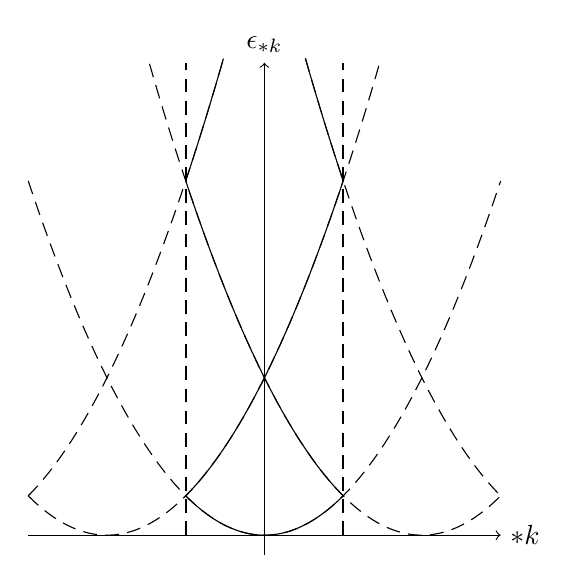
\begin{tikzpicture}
        
            % 动量横轴
            \draw[->] (-3,0) -- (3,0) node[right] {$\vb*{k}$};
            % 动能纵轴
            \draw[->] (0,-0.25) -- (0,6) node[above] {$\epsilon_{\vb*{k}}$};

            % 布里渊区边界
            \draw[dash pattern=on5pt off3pt, thick] (-1, 0) -- (-1, 6);
            \draw[dash pattern=on5pt off3pt, thick] (1, 0) -- (1, 6);
            
            % 画出布里渊区以外的能谱
            
            \draw[dash pattern=on5pt off3pt,samples=50, smooth, domain=-3:1.46] plot(\x,{0.5*((\x+2)*(\x+2))});
            \draw[dash pattern=on5pt off3pt,samples=50, smooth, domain=-3:3] plot(\x,{0.5*((\x)*(\x))});
            \draw[dash pattern=on5pt off3pt,samples=50, smooth, domain=-1.46:3] plot(\x,{0.5*((\x-2)*(\x-2))});
            \draw[dash pattern=on5pt off3pt,samples=50, smooth, domain=0.52:3] plot(\x,{0.5*((\x-4)*(\x-4))});
            \draw[dash pattern=on5pt off3pt,samples=50, smooth, domain=-3:-0.52] plot(\x,{0.5*((\x+4)*(\x+4))});

            % 画出布里渊区内部的$\epsilon_{\vb*{k}}$曲线,以及由于晶格周期性而导致的能谱平移
            \draw[samples=50, smooth, domain=-1:1] plot(\x,{0.5*(\x*\x)});
            \draw[samples=50, smooth, domain=-1:1] plot(\x,{0.5*((\x-2)*(\x-2))});
            \draw[samples=50, smooth, domain=-1:1] plot(\x,{0.5*((\x+2)*(\x+2))});
            \draw[samples=50, smooth, domain=0.52:1] plot(\x,{0.5*((\x-4)*(\x-4))});
            \draw[samples=50, smooth, domain=-1:-0.52] plot(\x,{0.5*((\x+4)*(\x+4))});
    
        \end{tikzpicture}
        
    }
    \subfigure[相互作用打开能隙,形成分离的能带]{
        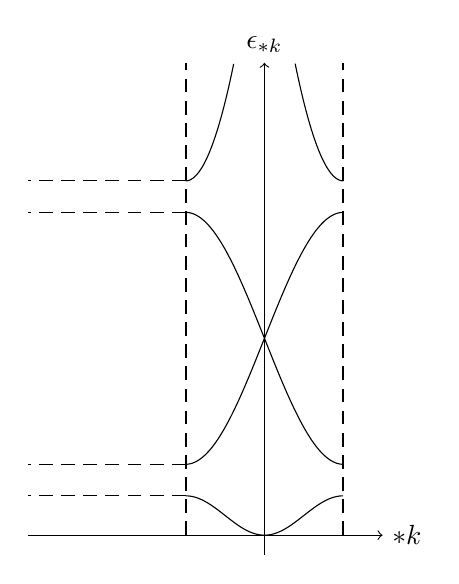
\begin{tikzpicture}
        
            % 动量横轴
            \draw[->] (-3,0) -- (1.5,0) node[right] {$\vb*{k}$};
            % 动能纵轴
            \draw[->] (0,-0.25) -- (0,6) node[above] {$\epsilon_{\vb*{k}}$};

            % 布里渊区边界
            \draw[dash pattern=on5pt off3pt, thick] (-1, 0) -- (-1, 6);
            \draw[dash pattern=on5pt off3pt, thick] (1, 0) -- (1, 6);
            
            % 画出布里渊区内部的$\epsilon_{\vb*{k}}$曲线,以及由于晶格周期性而导致的能谱平移
            \draw[samples=50, smooth, domain=-1:1] plot(\x,{0.25-0.25*cos(3.14*\x r)});
            \draw[samples=50, smooth, domain=-1:1] plot(\x,{2.5+1.6*sin(1.57*\x r)});
            \draw[samples=50, smooth, domain=-1:1] plot(\x,{2.5-1.6*sin(1.57*\x r)});
            \draw[samples=50, smooth, domain=0.39:1] plot(\x,{4.5+4*(\x-1)*(\x-1)});
            \draw[samples=50, smooth, domain=-1:-0.39] plot(\x,{4.5+4*(\x+1)*(\x+1)});

            % 标记能带和带隙
            \foreach \hei in {0.5, 0.9, 4.1, 4.5}
                \draw[dash pattern=on5pt off3pt] (-1,\hei) -- (-3, \hei);
    
        \end{tikzpicture}
        
    }
    \caption{能带结构}
    \label{fig:bloch-energy-band}
\end{figure}

具体“抹去奇异性”的方式可以通过一阶简并微扰论看出来。先考虑一个简单的一维的例子,设晶格常数为$a$,则周期性势场为
\[
    V(x) = \sum_n \ee^{\ii \frac{2 \pi}{a} n x}.
\]
在没有周期性势场时电子波函数就是一维无限深势阱中的形式:
\[
    \psi_n(x) = \frac{1}{\sqrt{L}} \ee^{\ii \frac{2 \pi n x}{L}},
\]
简并出现在$n$和$-n$之间。我们可以尝试做非简并微扰论,
% TODO

晶格动量就是把自由电子的广延动量挪到第一布里渊区中,因此也可以称为\concept{简约动量}。

\subsubsection{导电性分类}

晶体的导电性可以分类如下:
\begin{itemize}
    \item 绝缘体就是有电子的能带被完全填满的系统。
    \item 金属就是有一些有电子的能带只是部分被填满的系统。
    \item \concept{半金属}是一些有电子的能带只有少量电子的系统,其导电性不好,但是仍然呈现一些金属的性质。
    \item \concept{半导体}是掺杂了的绝缘体,如果杂质能够形成能量大体上是在满带顶附近的局域空穴态,以及能量大体上是在空带底附近的局域电子态,那么热涨落就会让一些电子填充进空带中,而让满带中出现空穴,这就同时形成了两种载流子。
    不能依靠热涨落让电子从满带跳往空带,因为这要求费米温度量级的温度;我们需要掺杂才能够形成半导体。
\end{itemize}

能带论能够解释为什么绝缘体不导电。自由电子气模型无法解释为什么绝缘体不导电——绝缘体中同样有大量的电子,似乎本应该导电。

\subsubsection{赝势}

离子实中的核心电子轨道和价电子轨道同时都是单电子哈密顿量的本征态:
\begin{equation}
    H \ket{\psi_c} = E_c \ket{\psi_c}, \quad H \ket{\psi_\text{v}} = E_\text{v} \ket{\psi_\text{v}},
\end{equation}
这里$c$标记了各个内层电子轨道。定义
\begin{equation}
    \ket{\psi_\text{v}^\text{ps}} = \ket{\psi_\text{v}} + \sum_c \ket{\psi_c} \braket*{\psi_c}{\psi_\text{v}^\text{ps}},
\end{equation}
则计算得到
\[
    (H - E_\text{v}) \ket{\psi_\text{v}^\text{ps}} = \sum_c (E_c - E_\text{v}) \ket{\psi_c} \braket*{\psi_c}{\psi_\text{v}^\text{ps}},
\]
从而
\begin{equation}
    \left(H - \sum_c (E_c - E_\text{v}) \dyad*{\psi_c}\right) \ket{\psi_\text{v}^\text{ps}} = E_\text{v} \ket{\psi_\text{v}^\text{ps}}.
\end{equation}
这意味着可以定义一个相较于晶体中实际的周期势要平滑得多的“势”
\begin{equation}
    V^\text{ps} = V - \sum_c (E_c - E_\text{v}) \dyad*{\psi_c},
\end{equation}
从这个势出发做计算能够得到正确的能谱。

\subsubsection{$\vb*{k} \cdot \vb*{p}$模型和有效质量}

设我们需要计算$\vb*{k}_0$附近电子的行为。定义
\begin{equation}
    \chi_{n \vb*{k}}(\vb*{r}) = \ee^{\ii (\vb*{k} - \vb*{k}_0) \cdot \vb*{r}} \psi_{n \vb*{k}} ,
\end{equation}
能够验证正交性和完备性均成立,即$\chi_{n \vb*{k}}$构成晶体中电子的一组正交完备基底。

\begin{equation}
    H = \frac{\vb*{p}^2}{2m} + V(\vb*{r}) + \frac{\vb*{k}^2}{2m} + \frac{\vb*{k} \cdot \vb*{p}}{m},
\end{equation}
因此做微扰论能够得到

\begin{equation}
    \frac{1}{m_l} = \sum_m 
\end{equation}

能带越宽,有效质量越轻,能带越窄,有效质量越重。\concept{重费米子系统}指的是有效质量非常大的系统,从而这样的系统基本上是强关联系统。

Luttinger模型:能带反转?

\subsection{从紧束缚模型出发得到的模型}

\subsubsection{紧束缚模型}

最后考虑一个极限情况。假定晶格的吸引作用是如此之强,以至于电子是高度定域的,这样只有最近邻的格点之间才会跃迁。
进一步,考虑一个单能带的低能有效理论,就得到
\begin{equation}
    {H} = - \sum_{\pair{i, j}} (t_{ij} {c}^\dagger_i {c}_j + \text{h.c.}).
\end{equation}
这称为\concept{紧束缚模型}。如果满足平移不变性,就有
\begin{equation}
    {H} = - \sum_{\pair{i, j}} (t {c}^\dagger_i {c}_j + \text{h.c.}).
\end{equation}

\subsubsection{单能带系统}

对单带模型,在Wannier表象下,库仑相互作用可以表示成如下矩阵元形式:
\begin{equation}
    \begin{aligned}
        H_{i i' j' j} &= \frac{1}{2} \int \dd[3]{\vb*{r}} \int \dd[3]{\vb*{r}'} \braket{i}{\vb*{r}} \braket{i'}{\vb*{r}'} V(\vb*{r} - \vb*{r}') \braket{\vb*{r}'}{j'} \braket{\vb*{r}}{j} \\
        &= \frac{1}{2} \int \dd[3]{\vb*{r}} \int \dd[3]{\vb*{r}'} w_i^*(\vb*{r}) w_{i'}^*(\vb*{r}') V(\vb*{r} - \vb*{r}') w_{j'}^*(\vb*{r}') w_j^*(\vb*{r}),
    \end{aligned}
    \label{eq:wannier-basis-interaction}
\end{equation}
于是总的哈密顿量为
\begin{equation}
    H = \sum_{i, i', \sigma} c^\dagger_{i \sigma} t_{i i'} c_{j \sigma} + \sum_{i, i', j, j', \sigma, \sigma'} V_{i i' j' j} c^\dagger_{i \sigma} c^\dagger_{i' \sigma'} c_{j' \sigma'} c_{j \sigma}.
\end{equation}

上面的哈密顿量是最为一般的,原则上可以描述一切晶体中的电子系统。
例如,原则上,自由电子气可以通过引入非常远的跃迁矩阵元来实现。
在我们假定电子真的只存在最近邻跃迁时,我们有
\begin{equation}
    \sum_{i, i', \sigma} c^\dagger_{i \sigma} t_{i i'} c_{j \sigma} = \sum_{\pair{i, j}, \sigma} t_{ij} c^\dagger_{i \sigma} c_{j \sigma}.
\end{equation}
我们称满足这个条件的自由电子模型为\concept{紧束缚模型}。我们当然还可以引入次近邻跃迁等来修正紧束缚模型。

如果只有最近邻或是次近邻的跃迁,那么我们就有一个非常直观的物理图像:似乎可以用“某个电子正在某个格点附近”来标记一个电子,即电子似乎被紧紧地束缚在晶格上,无法长距离移动,这就是“紧束缚”一词的来历。
或者,也有可能电子并不是特别局域,但是原子间距很大,以至于在系统中电子通常具有的动能下,非常远距离的跃迁似乎无法一次完成。
这就是说,紧束缚模型中,电子的动能不应该能够到达特别大,从而不应该有太大的能带带宽。

与自由电子气模型或凝胶模型不同,紧束缚模型对相互作用是非常敏感的,不能保证加入(即使比较弱的)相互作用后,系统能够用费米液体理论描述,也不能保证能带论仍然有效。
这是出于一个非常直观的原因:紧束缚模型的能带通常更窄,从而态密度更大,从而库伦散射更明显,从而也更加容易在相互作用加入之后变成强关联系统。
或者,我们也可以如此理解紧束缚模型对相互作用的敏感性:由于电子动能不能取特别大的值,相比之下相互作用能量应该占据主导,从而系统具有强关联效应。

总之,以下几个说法基本上是等价的:
\begin{enumerate}
    \item 系统可以用紧束缚模型或者考虑了次近邻、再次近邻的紧束缚模型加上一个相互作用项描述;
    \item 系统中的电子跃迁能力不大;
    \item 系统能带不宽;
    \item 系统中电子动能有较低的上限。
\end{enumerate}
满足这些条件的模型通常对相互作用更加敏感,也更加容易出现强关联效应。
这就导致了一个非常有趣的现象:一些数值计算方法,如DMRG,需要将所有自由度都定义在晶格上,从而,它们可以毫无困难地用于模拟很大一类强关联系统,但是却无法用于有效地模拟普通的费米液体系统。

需要注意,并非所有强关联系统都出现在紧束缚模型中。费米液体系统加入了适当的相互作用之后也可以出现强关联效应,此时使用基于格点的计算方法就不能获得很好的效果了。

原则上$U_{i i' j' j}$对很多不同的$i, i', j', j$组合都有非零值。物理上这是很好理解的,因为库伦相互作用可以将任意原子附近的两个电子散射到任意的其它地方,由于高度定域的电子动量不确定,这里无所谓动量守恒的约束。
然而,由于只有原子间距很大时,紧束缚模型才成立,实际上,足够大的矩阵元的$i, i', j', j$中,$j$和$j'$不是最近邻,就是完全一样(即所谓on-site repulsion)。
由于Wannier波函数高度定域,从\eqref{eq:wannier-basis-interaction}中可以看出,仅有的可能是$i=i'=j=j'$,或是$i=j \neq i'=j'$,或是$i=j' \neq i' = j$。
于是就有
\[
    \begin{aligned}
        &\quad \sum_{i, i', j, j', \sigma, \sigma'} V_{i i' j' j} c^\dagger_{i \sigma} c^\dagger_{i' \sigma'} c_{j' \sigma'} c_{j \sigma} \\
        &= \sum_{i, \sigma, \sigma'} V_{iiii} c^\dagger_{i \sigma} c^\dagger_{i \sigma} c_{i \sigma} c_{i \sigma} 
        + \sum_{i, j, \sigma, \sigma'} V_{i j j i} c^\dagger_{i \sigma} c^\dagger_{j \sigma'} c_{j \sigma'} c_{i \sigma}
        + \sum_{i, j, \sigma, \sigma'} V_{i j i j} c^\dagger_{i \sigma} c^\dagger_{j \sigma'} c_{i \sigma'} c_{j \sigma},
    \end{aligned}
\]
第一项为
\[
    \begin{aligned}
        \sum_{i, \sigma, \sigma'} V_{iiii} c^\dagger_{i \sigma} c^\dagger_{i \sigma} c_{i \sigma} c_{i \sigma} &= 2 \sum_{i} V_{iiii} n_{i \uparrow} n_{i \downarrow} + \sum_{i} U_{iiii} n_i \\
        &= \sum_{i} U_i n_{i \uparrow} n_{i \downarrow} + \frac{1}{2} \sum_{i} U_{i} n_i,
    \end{aligned}
\]
这里我们重新定义
\begin{equation}
    U_i = 2 V_{iiii}.
\end{equation}
第二项实际上是密度-密度相互作用,即为
\[
    \sum_{i, j, \sigma, \sigma'} V_{i j j i} c^\dagger_{i \sigma} c^\dagger_{j \sigma'} c_{j \sigma'} c_{i \sigma} = \sum_{\pair{i, j}} V_{ij} n_i n_j,
\]
其中我们重新定义了$V_{ij} = V_{ijji}$。使用公式
\[
    \vb*{\sigma}_{\alpha \beta} \cdot \vb*{\sigma}_{\alpha' \beta'} = 2 \delta_{\alpha \beta'} \delta_{\beta \alpha'} - \delta_{\alpha \beta} \delta_{\alpha' \beta'},
\]
可以验证
\[
    \sum_{i, j, \sigma, \sigma'} V_{i j i j} c^\dagger_{i \sigma} c^\dagger_{j \sigma'} c_{i \sigma'} c_{j \sigma} = - 2 \sum_{\pair{i, j}} V_{i j i j} \left( \vb*{S}_{i} \cdot \vb*{S}_j + \frac{1}{4} n_i n_j \right).
\]
我们把上式右边的第二项吸收进$V_{ij}$中,并且重新定义$2V_{ijij}=J_{ij}$,于是总的相互作用哈密顿量就是
\[
    \sum_{i} U_i n_{i \uparrow} n_{i \downarrow} + \sum_{\pair{i, j}} V_{ij} n_i n_j - \sum_{\pair{i, j}} J_{i j} \vb*{S}_{i} \cdot \vb*{S}_j + \sum_{i} U_i n_i.
\]
由空间平移对称性,on-site repulsion肯定是均一的,这样我们可以将$\sum_i U_i n_i$丢进化学势中;而如果它不是均一的,就意味着系统实际上不具有完美的离散平移对称结构,即系统中存在无序,直观地看,就是散布的杂质对电子产生散射,这基本上是一个单体算符,于是我们就得到了紧束缚模型最一般的哈密顿量:
\begin{equation}
    H = - \sum_{\pair{i, j}, \sigma} t_{ij} c^\dagger_{i \sigma} c_{j \sigma} 
    + \sum_{i} U_i n_{i \uparrow} n_{i \downarrow} 
    + \sum_{\pair{i, j}} V_{ij} n_i n_j - \sum_{\pair{i, j}} J_{i j} \vb*{S}_{i} \cdot \vb*{S}_j 
    - \mu \sum_i n_i + \sum_{i, j, \sigma, \sigma'} \epsilon_{ij\alpha \beta} c^\dagger_{i \alpha} c_{j \beta}.  
\end{equation}
这里的每一项都是有意义的,从左到右分别是:
\begin{enumerate}
    \item 动能项,衡量电子在格点之间跳跃的可能性;
    \item on-site repulsion,仅考虑这个相互作用得到的模型是所谓\concept{Hubbard模型};
    \item 密度-密度相互作用项,可能导致系统中出现持续的、不能平息的电子密度涨落,即所谓电荷密度波;
    \item 自旋-自旋相互作用项,可能导致出现自旋密度波,这一项意味着在有多个轨道的情况下,每个轨道上放置一个电子,且所有电子的自旋都平行时,系统能量最低,这就是所谓洪特规则;
    \item 化学势,调节系统中电子个数;
    \item 无序,可能来自杂质或是晶格的缺陷。
\end{enumerate}

\subsubsection{多能带的情况}

以上的讨论集中在单能带模型中;多个能带的情况允许一些新的能带之间的相互作用通道。

实际的原子内部的洪特规则应该就是在这里能够拿到

\subsubsection{Wannier波函数和原子电子轨道}

本节展示一个极端情况。我们假设原子周围的电子轨道是如此局域,以至于
\begin{equation}
    \int \dd[3]{\vb*{r}} \varphi_i^*(\vb*{r}) \varphi_j(\vb*{r}) = \delta_{ij},
\end{equation}
则

TODO:单带模型中轨道波函数就是Wannier波函数

可以先假装轨道波函数真的是Wannier波函数,然后做杂化

总之,在原子轨道波函数之间真的没有什么交叠的情况下,原子轨道波函数就是Wannier波函数。
然而,在大多数情况下,原子轨道波函数还是比较不局域的,我们需要先从原子轨道波函数出发计算得到Bloch波函数,然后做傅里叶变换得到比原子轨道波函数更加局域的Wannier波函数。

\subsection{金属和朗道费米液体}

本节处理带有相互作用的系统。金属中存在可以四处移动的巡游电子,这些电子之间存在库伦排斥,而又有晶格对电子施加周期势。
先考虑周期势的影响,裸电子将会有能量修正而成为能带电子,无相互作用的能带电子组成费米气体,很容易处理。
库伦排斥和声子介导的吸引相互作用合并为电子-电子相互作用,非常难以处理——电子-电子相互作用可以导致各种奇特的现象,并且其量级通常与费米能的量级一致。
然而,金属的行为在很多方面非常像费米气体,这意味着实际上描述金属的低能有效理论基本上就是一个费米气体加上一定的相互作用。
\concept{朗道费米液体}是一个这样的低能有效理论,其基本假设为:
\begin{enumerate}
    \item 费米液体的状态可以和费米气体一样,使用某种费米子的占据数标记,并且系统能量可以写成占据数的函数。
    这个假设对哈密顿量的形式做出了很强的限制,因为此时的哈密顿量已经在粒子数表象下被严格对角化了。(但是这个哈密顿量仍然可以不是自由哈密顿量,因为可以有密度-密度相互作用)不过我们将会看到,这样的限制是合理的。
    \item 当相互作用趋于零(“被关闭”)时,费米液体态回退到实际的费米气体态,我们假设此时费米液体态的占据数和实际的费米气体态的占据数相同。
    这个假设实际上是说,费米液体中的占据数所描述的准粒子实际上是经过某种重整化的电子,和电子可以一一对应。
\end{enumerate}

可以通过这样的方式想象费米液体可以怎样产生:对无相互作用的能带电子%
\footnote{
    应当注意能带电子这个名称本身有些模糊不清。只计算周期性势场的影响可以得到能带,只计算经过平滑处理的赝势也可以得到能带,将一部分相互作用作为自能修正而留下最为显著的相互作用通道作为碰撞也可以得到能带(虽然还需要额外计算碰撞的影响,如费米液体中那样),对很多系统,其实相互作用全都考虑进去了还是可以得到能带——如同用DFT计算出来的那样。
    例如,在费米液体中,如果粒子数涨落不大,完全可以用粒子数平均值代替相互作用项中的准粒子占据数。
    即使相互作用大一些,也可以理解成“能带被拉歪了”。
}%
,我们可以浸染地将相互作用加入,如果没有出现诸如费米子配对之类的情况,那么第二个假设就已经满足了。
相互作用会导致电子出现自能修正,由于库仑相互作用的顶角是保持粒子数守恒的,不存在一个电子衰变成多个其它粒子的过程,因此自能修正是实数,即单电子态的确是本征态。%
\footnote{
    虽然如此,如果我们将高于费米面的电子称为电子而将低于费米面的电子称为空穴,那么的确可以出现一个电子和费米球中的空穴发生相互作用,而衰变成电子和空穴的过程。
    见\autoref{sec:fermi-liquid-ground}。
}%
在很多粒子数守恒的理论——如$\phi^4$理论或是QED——中,可以有稳定的单粒子、二粒子、三粒子……本征态,虽然$n$粒子态的能量不是$n$个粒子的能量简单相加,但是无论如何,一个本征态的能量可以写成各个动量上的粒子的占据数的函数,因此量子态可以用占据数标记,能量也可以用粒子数标记,即第一个假设也是成立的。

在什么情况下费米液体理论失效?如果相互作用是吸引的,那么低温下可能出现费米子配对,此时总是会出现相变。
我们将在\autoref{sec:low-and-super}中讨论这种情况。
如果相互作用较强,能带的图像可能就完全不适用了,此时系统的元激发可能都不是经过修正的电子,也无所谓费米液体。
如果有一些不能写成粒子数算符乘积的相互作用通道,费米液体理论同样不成立
令人震惊的是,虽然大部分实际体系中库仑相互作用的确很强,费米液体图像仍然是适用的。

由于费米液体中的准粒子是电子的单体激发,可以从费米液体中准粒子的行为中看到很明显的普通电子的影子,由于准粒子场和电子场的对称性相同,准粒子也是费米子,准粒子能谱和电子能谱形式类似,自旋均为$1/2$,带电量相同,等等。
唯象的讨论中可以直接将费米液体中的准粒子当成电子。

\subsubsection{基态附近的激发}\label{sec:fermi-liquid-ground}

与高能物理中不同,实际的凝聚态体系的基态中都有大量准粒子。由于准粒子是费米子,系统基态中有一个费米球。
由于粒子数守恒,系统基态附近的激发态就是一些准粒子从费米球内部被打到费米球外部之后形成的,并且距离费米面均不远。
这样,我们可以忽略费米海而认为系统中实际上有两种元激发:“电子”和“空穴”。
实际上,在费米液体理论中通常也只分析费米面附近的物理,部分原因在于费米海的结构可以非常复杂,因此只考虑费米面附近的物理是比较容易的,也是比较有实际意义的(因为是低温近似),部分原因在于只有这里才确定有稳定的准粒子——通常准粒子的寿命在接近费米面时比较长,因此看起来像是“真正的”粒子(否则会有非常明显的能级展宽)。

这件事的原因如下。首先应当注意,虽然准粒子的自能修正总是实数,从而,在没有其它任何准粒子时,单个准粒子可以永远稳定存在而不会衰变,但与高能物理中的情况不同,费米球的存在意味着如果费米面上方出现了一个准粒子,它会激发费米海内部的准粒子,从而产生一个空穴。
因此,在基态(不是真空态,而是带有费米球的态),费米面上方的准粒子的确会发生衰变。
将费米面上方的准粒子和费米球内部的空穴看成两种元激发可以更加清楚地看到这一点:此时费米面上方的准粒子的个数根本不是守恒的(从而,积掉费米海会产生一个非幺正的理论),从而其自能修正不可能是实数。

设准粒子寿命为$\tau$,则$\tau$反比于散射速率,而散射速率正比于库仑相互作用的强度。完整地做这个计算是很困难的,因为涉及到静电屏蔽等复杂的效应。
由于我们只做数量级估计,暂时将寿命对整个费米面做平均,从而使用一个常数$M$表示相互作用强度。
散射的过程可以概括为:一个动量为$\vb*{p}$的费米面外部的粒子(实际上是费米液体中的准粒子,下同)的能量降低,变成了动量为$\vb*{p}_1$的粒子,同时激发了一个费米面内的动量为$\vb*{p}_2$的粒子。
结果是,动量为$\vb*{p}$的费米面以外的粒子衰变成了两个粒子,动量分别为$\vb*{p}_1$和$\vb*{p} - \vb*{p}_1 + \vb*{p}_2$,还有一个动量为$\vb*{p}_2$的空穴。
设动量分别为$\vb*{p}_1$和$\vb*{p} - \vb*{p}_1 + \vb*{p}_2$的两个粒子和动量为$\vb*{p}_2$的空穴的总态密度在当前温度下的期望值为$n$,由费米黄金法则有
\[
    \frac{1}{\tau} \propto \text{transition rate} \sim \abs{M}^2 n.
\]
由于系统中的粒子非常多,不同能级上粒子数的涨落可以略去,即认为不同能级上不多不少正好就有费米-狄拉克分布给出的粒子个数,%
\footnote{这是热力学系统的一般性质:系统规模大时涨落可略去。由于本文涉及的系统都是多体系统,总是可以做这样的近似。}%
那么就有
\[
    n = \int \dd[3]{\vb*{p}_1} \int \dd[3]{\vb*{p}_2} (1 - f(\epsilon_{\vb*{p}_1})) f(\epsilon_{\vb*{p}_2}) (1 - f(\epsilon_{\vb*{p} - \vb*{p}_1 + \vb*{p}_2})) \delta(\epsilon_{\vb*{p}} - \epsilon_{\vb*{p}_1} + \epsilon_{\vb*{p}_2} - \epsilon_{\vb*{p} - \vb*{p}_1 + \vb*{p}_2}).
\]
因子$(1-\epsilon_{\vb*{p}_1})$表示动量为$\vb*{p}_1$的粒子应该占据一个空态(或者说在接近零温时应该在费米面以外),因子$f(\epsilon_{\vb*{p}_2})$表示空穴一定来自一个已有的粒子,最后的$\delta$函数强制要求能量守恒。
我们不严格计算这个积分,而是做一些数量级估计。
由于$\vb*{p}_2$在费米面以下而$\vb*{p}- \vb*{p}_1 + \vb*{p}_2$在费米面以上,容易写出以下不等式
\[
    0 < \xi_{\vb*{p}_1} < \xi_{\vb*{p}}, \quad 0 < - \xi_{\vb*{p}_2} < \xi_{\vb*{p}} - \xi_{\vb*{p}_1} < \xi_{\vb*{p}},
\]
对$n$有贡献的$\vb*{p}_1$和$\vb*{p}_2$均满足这些不等式,这些不等式给出了两个宽度为$\xi_{\vb*{p}}$的球壳,因此
\[
    n \leq (4 \pi k_\text{F}^2 \xi_{\vb*{p}})^2,
\]
于是
\begin{equation}
    \frac{1}{\tau} \lesssim \xi_{\vb*{p}}^2.
\end{equation}
因此,如果准粒子非常接近费米液体的费米面,那么它是非常稳定的,因为此时$\xi_{\vb*{p}}$很小。从物理图像上看,此时的准粒子虽然会和费米海中的准粒子发生相互作用,但其能量不足以产生粒子-空穴对,因此也不会衰变。

粒子“稳定”的数值判据是什么?按照费米-狄拉克分布,$\expval*{{n}}$在$\epsilon_\text{F}$附近一个大约长为$T$的区域内明显偏离阶跃函数;另一方面,由于相互作用能量本身会有一个弥散,为
\[
    \Delta E \sim \frac{1}{\Delta t} \sim \frac{1}{\tau},
\]
其中$\tau$为准粒子平均自由时间。粒子稳定意味着
\[
    \Delta E \ll \frac{1}{T},
\]
也即
\[
    \frac{1}{\tau} \ll T.
\]
准粒子平均自由时间本身和温度有关,它大约是单位时间发生碰撞的概率的倒数,而只有费米子附近准粒子数明显偏离阶跃函数的那一部分准粒子比较有可能发生碰撞(费米球内部的准粒子不怎么会被激发,费米球外面根本没有准粒子),因此
\[
    \frac{1}{\tau} \sim T^2,
\]
最后就发现我们有
\[
    T \ll 1.
\]
因此费米液体图像只在低温下适用。

% TODO
然而,设$\Delta x$为准粒子坐标的不确定度,数量级上有
\[
    \frac{1}{\Delta x} \sim \frac{1}{\Delta t} \sim \Gamma,
\]
其中$\Gamma$是单位时间的散射几率,而我们又有
\[
    \Delta p \Delta x \sim \hbar,
\]
那么就有
\[
    \Delta p \sim \Gamma.
\]
由于准粒子散射是二体过程,在低温下$\Gamma$正比于$\expval*{{n}}$在$\epsilon_\text{F}$附近明显偏离阶跃函数的区域的厚度的平方。
可以证明低温下这确实是正确的。

总之,准粒子之间的碰撞不可忽略意味着费米面以上的准粒子会衰变。
然而,在费米面附近,这种衰变是非常缓慢的,以至于我们可以认为任何一种动量确定的准粒子分布都可以长期稳定存在,即哈密顿量在以动量标记的粒子数表象下是对角化的。
因此,费米液体的能级结构和费米气体完全一致。

\subsubsection{哈密顿量和相互作用形式}

然而,费米液体的能级结构和费米气体完全一致并不意味着电子之间的相互作用完全不产生任何影响,因为每个能级具体的能量大小可以经历修正。
此外,即使电子之间的相互作用可以忽略,向系统加入或取出电子也会让费米球发生变化,从而让系统总能量平摊到每个准粒子上的份额发生变化。
这意味着准粒子的哈密顿量并不是简单的
\[
    H = \sum_{\vb*{k}, \sigma} \epsilon_{\vb*{k}} n_{\vb*{k} \sigma},
\]
而有一些高阶项,它们表示密度-密度相互作用。

考虑一个能量本征态,其中准粒子在费米面之上的数量为$\var{n}$($\delta$表示相对基态的偏离,正表示有粒子,负表示有空穴)。
考虑到费米液体理论的第一条假设,把能量本征值相对于零温平衡态(由于费米海的结构可以非常复杂,零温能量反而是算不出来的,我们也不需要计算它)的变化写成以下级数展开($\vb*{k}$在费米面附近):
\begin{equation}
    \var{E} = \underbrace{\sum_{\vb*{k}, \sigma} \epsilon^0_{\vb*{k}} \var{n_{\vb*{k} \sigma}}}_{\var{E_1}} + \underbrace{\frac{1}{2V} \sum_{\vb*{k}, \vb*{k}', \sigma, \sigma'} f_{\sigma \sigma' \vb*{k} \vb*{k}'} \var{n_{\vb*{k} \sigma}} \var{n_{\vb*{k}' \sigma'}}}_{\var{E_2}},
    \label{eq:fermi-liquid-energy}
\end{equation}
其中$\var{n}$表示准粒子数目相对基态的变化。把能量写成粒子数的函数假定了自旋守恒。对动量做求和化积分,就得到
\begin{equation}
    \frac{\var{E}}{V} = \underbrace{\sum_{\sigma} \int \frac{\dd[3]{\vb*{k}}}{(2\pi)^3} \epsilon^0_{\vb*{k}} \var{n_{\vb*{k} \sigma}}}_{\var{E_1} / V} + \underbrace{\frac{1}{2} \sum_{\sigma, \sigma'} \int \frac{\dd[3]{\vb*{k}}}{(2\pi)^3} \int \frac{\dd[3]{\vb*{k}'}}{(2\pi)^3} f_{\sigma \sigma' \vb*{k} \vb*{k}'} \var{n_{\vb*{k} \sigma}} \var{n_{\vb*{k}' \sigma'}}}_{\var{E_2} / V}
\end{equation}
我们保留到二阶项,一阶项给出准粒子的自由理论,二阶项给出准粒子的相互作用。
这种相互作用并不会让粒子数发生涨落或是让单个准粒子的动量发生涨落,而只会对能级做修正,是所谓的“前向散射”。

重整化群可能给出更高阶项,而也许二阶项实际上可以忽略,而绕了一大圈之后发现$\abs{M}$很小,从而实际上在很大的区域内费米液体图像均适用。
为了表明我们保留到二阶项是正确的,我们给出一个数量级估计,说明一阶项和二阶项的量级是同阶的,而低于更高阶项。
我们知道由于相互作用的存在,总能量$E$肯定不是单粒子哈密顿量(比如说$k^2/2m$这种形式)的期望值简单加起来的结果,但是显然能量具有可加性,设想我们改变了准粒子数分布,这样应该有
\[
    \var{E} = \sum_{\vb*{k}, \sigma} \epsilon_{\vb*{k} \sigma} \var{n_{\vb*{k} \sigma}},
\]
其中$\epsilon_{\vb*{k}}$是在有限温度下的近平衡态激发一个准粒子的能量,它的一部分是单准粒子能量,一部分是其它准粒子给它的相互作用能之和。
因此,$\epsilon_{\vb*{k}}$会依赖准粒子数分布。由于我们只研究二体相互作用,我们有
\[
    \epsilon \sim \sum_{\vb*{k}'} \text{something} \cdot n_{\vb*{k}'},
\]
于是设
\[
    \var{\epsilon_{\vb*{k} \sigma}} = \frac{1}{V} \sum_{\vb*{k}', \sigma'} f_{\sigma \sigma' \vb*{k} \vb*{k}'} \var{n_{\vb*{k}' \sigma'}},
\]
记$\epsilon_{\vb*{k}}^0$为$n_{\vb*{k}}$一概为零的$\epsilon_{\vb*{k}}$,代入$\var{E}$中就得到\eqref{eq:fermi-liquid-energy};第二项的$1/2$因子是因为一对粒子会被计数两次,所以要除以$2$;由于我们假定准粒子分布相对于零温只有微小的偏离,$\epsilon_{\vb*{k}}$被取为零温的值。
虽然$\epsilon^0 \var{n}$看起来比$f\var{n} \var{n}$大,但需要注意到我们在巨正则系综中工作,则真的有意义的应该是$E-\mu N$(且由于是近平衡,应有$\var{E} = \mu \var{N}$),而
\[
    \sum_{\vb*{k}} (\epsilon^0_{\vb*{k}} - \mu) \var{n_{\vb*{k}}} \sim \var{n}^2,
\]
于是$\epsilon^0 \var{n}$项和$f\var{n} \var{n}$项的贡献是同阶的,都需要考虑。
更高阶相互作用则涉及$\var{n}$的更高阶项,于是不考虑。因此,\eqref{eq:fermi-liquid-energy}的确是成立的。

在已经知道了$E$的表达式之后(比如说微扰计算出了体系能量),可以用变分计算出各个物理量:
\begin{equation}
    \epsilon_{\vb*{k}} = \fdv{E}{n_{\vb*{k} \sigma}} , \quad f_{\sigma \sigma' \vb*{k} \vb*{k}'} = V \frac{\var[2]{E}}{\var{n_{\vb*{k} \sigma}}\var{n_{\vb*{k}' \sigma'}}}, \quad \mu = \pdv{E}{N}.
\end{equation}

\eqref{eq:fermi-liquid-energy}中的一阶项可以看成一个等效的单粒子能量。由于只讨论费米面附近的理论,我们让能量从费米面量起,即使用$\xi$代替$\epsilon$,$k=k_\text{F}$时$\xi^0_{\vb*{k}}$就是零,在假定费米面具有旋转对称性的情况下可以做展开
\[
    \xi^0_{\vb*{k}} = \frac{k_\text{F}}{m^*} (k - k_\text{F}).
\]
我们仿照自由粒子的能量
\[
    \xi_{\vb*{k}} = \frac{k^2}{2m} - \frac{k_\text{F}^2}{2m} \approx \frac{k_\text{F}}{m} (k - k_\text{F})
\]
得到了一个等效质量$m^*$。能够像上面这样做的前提是准粒子能谱要足够光滑,如果像声子那样,就没法定义任何等效质量。%
\footnote{应注意此处的等效质量和“激发有能隙,是有质量的”中的“质量”是不同的;前者并不代表有一个能隙,而只是$\epsilon_{\vb*{k}}$的$k^2$项的系数而已。}%
如果温度很高,以至于不能保证有趣的行为仅仅发生在费米面附近,那有效质量的概念也没有什么用;实际上此时费米液体的理论就没有什么用。
请注意\eqref{eq:fermi-liquid-energy}完全是形式上的:诸如晶格势能造成的单粒子能量修正已经被纳入了$\var{E_1}$中,而只要费米面保持旋转对称性,就可以引入等效质量的概念。
并且,在只有费米面附近才有明显的激发的情况下,可以不失一般性地设
\[
    \epsilon_{\vb*{k}}^0 = \frac{k^2}{2m^*},
\]
因为真正有意义的是$\epsilon_{\vb*{k}} - \mu$,只需要同时调节$\epsilon_{\vb*{k}}$和$\mu$就可以让准粒子的$\epsilon_{\vb*{k}}$取自由粒子的形式。
再次强调,调节$\epsilon_{\vb*{k}}$和$\mu$之类的操作只适用于费米面附近;因此对一个费米液体我们通常避免讨论费米球深处有什么——这些东西对费米面附近的行为并不重要。

对二阶项,假定系统具有自旋旋转不变性,则$f$的取值完全由$f_{\uparrow \uparrow \vb*{k} \vb*{k}'}$和$f_{\uparrow \downarrow \vb*{k} \vb*{k}'}$决定。
实际上,由于$\vb*{k}$局限在费米面附近,我们有
\[
    f_{\alpha \beta \vb*{k} \vb*{k}'} = f_{\alpha \beta}(\vartheta),
\]
$\vartheta$是$\vb*{k}$和$\vb*{k}'$的夹角。这样,设
\begin{equation}
    \begin{aligned}
        f_{\uparrow \uparrow}(\vartheta) &= f^\text{S}(\vartheta) + f^\text{A}(\vartheta), \\
        f_{\uparrow \downarrow}(\vartheta) &= f^\text{S}(\vartheta) - f^\text{A}(\vartheta),
    \end{aligned}
\end{equation}
或者等价地可以设
\begin{equation}
    {f}(\vartheta) = f^\text{S}(\vartheta) + {\sigma} {\sigma}' f^\text{A}(\vartheta)
\end{equation}
从而将自旋守恒这一事实一并表示出来(${\sigma}^z$就是$z$方向的泡利矩阵),并将$f^\text{S}(\vartheta)$和$f^\text{A}(\vartheta)$展开成无量纲常数:
\begin{equation}
    \frac{k_\text{F} m^*}{\pi^2} f^\text{S,A}(\vartheta) = \sum_{l=0}^\infty F_l^\text{S,A} \legpoly (\cos \vartheta).
\end{equation}
于是,给定参数$m^*$,$k_\text{F}$以及$\{F_l^\text{S,A}\}$,费米液体服从的物理规律就给定了。
在这里,我们实际上又把准粒子当成了可以彼此散射、有相互作用的粒子,“准粒子动能”$k^2/2m^*$和“准粒子势能”$f_{\alpha \beta}(\vartheta)$是“单个准粒子能量”$\epsilon_{\vb*{k}}$的两部分;单单一个$k^2/2m^*$肯定和$\epsilon_{\vb*{k}}$是不一样的。

实际上,如果一个费米液体系统可以确定是一个实际的费米气体加入相互作用的结果,并且如前所述,能够保证准粒子个数和实际费米子的个数一样,自旋相同,等等,并且保证自旋旋转不变性、空间平移不变性、空间各向同性,那么费米液体中准粒子的等效质量和实际费米子的质量有一个简单的,使用$\{F_l^\text{S,A}\}$写出的关系。
由于
\[
    E - E_0 = \sum_{\vb*{k}} \var{n_{\vb*{k}}} \epsilon_{\vb*{k}},
\]
由动量为$\vb*{k}$的一个准粒子的运动速度为
\[
    \vb*{v}_i = \pdv{E}{\vb*{p}_i} = \pdv{\epsilon_{\vb*{k}}}{\vb*{k}},
\]
上式的量子版本就是
\[
    {\vb*{v}} = \pdv{{\epsilon}_{\vb*{k}}}{\vb*{k}}.
\]
我们于是可以将${\vb*{v}}$当成费米液体中准粒子的流速。设$\rho$是某种守恒荷的密度,则任意一个流算符的期望可以写成
\[
    \begin{aligned}
        \expval*{\rho \vb*{v}} = V \int \frac{\dd[3]{\vb*{k}}}{(2\pi)^3} \expval{\rho \pdv{{\epsilon}}{\vb*{k}}} , 
    \end{aligned}
\]
准粒子和实际的费米子数量相同,准粒子的粒子数流密度算符就是实际费米子的粒子数流密度算符,且由于动量守恒,一个准粒子的总动量就是与它对应的实际费米子的总动量%
\footnote{
    可以这样论证这件事:在关闭相互作用时费米液体“无缝地”退化到实际的费米气体上,因此在无相互作用点处费米液体中准粒子的动量就是实际粒子的动量。
    现在缓慢地加上相互作用,则费米液体准粒子的动量可以发生连续变化,但有限体系中动量实际上是分立的,从而动量只能不变。
}%
% TODO:这里的推导细节有问题
,而实际费米子的总动量就是总质量流(因为$\vb*{p}=m\vb*{v}$);由于动量和自旋守恒,我们将费米子占据数算符用$\vb*{k}$和$\sigma$标记,于是我们有
\[
    \sum_{\vb*{k}, \sigma} \int \frac{\dd[3]{\vb*{k}}}{(2\pi)^3} \vb*{k} {n}_{\vb*{k} \sigma} = \trace \int \frac{\dd[3]{\vb*{k}}}{(2\pi)^3} m \pdv{{\epsilon}}{\vb*{k}} {n}.
\]
同样${\epsilon}$也适用一样的推导,于是就有
\[
    \int \frac{\dd[3]{\vb*{k}}}{(2\pi)^3} m \pdv{\epsilon_{\vb*{k} \sigma}}{\vb*{k}} n_{\vb*{k} \sigma} = \int \frac{\dd[3]{\vb*{k}}}{(2\pi)^3} \vb*{k} n_{\vb*{k} \sigma},
\]
对上式求变分,就有
\[
    \begin{aligned}
        \int \frac{\dd[3]{\vb*{k}}}{(2\pi)^3} \vb*{k} \var{n_{\vb*{k} \sigma}} &= \var \int \frac{\dd[3]{\vb*{k}}}{(2\pi)^3} m \pdv{\epsilon_{\vb*{k} \sigma}}{\vb*{k}} n_{\vb*{k} \sigma} \\
        &= m \int \frac{\dd[3]{\vb*{k}}}{(2\pi)^3} \pdv{\epsilon_{\vb*{k} \sigma}}{\vb*{k}} \var{n_{\vb*{k} \sigma}} + m \int \frac{\dd[3]{\vb*{k}}}{(2\pi)^3} \int \frac{\dd[3]{\vb*{k}'}}{(2\pi)^3} n_{\vb*{k} \sigma} \var{n_{\vb*{k}' \sigma}} \pdv{f_{\sigma}(\vartheta)}{\vb*{p}} \\
        &= m \int \frac{\dd[3]{\vb*{k}}}{(2\pi)^3} \pdv{\epsilon_{\vb*{k} \sigma}}{\vb*{k}} \var{n_{\vb*{k} \sigma}} - m \int \frac{\dd[3]{\vb*{k}}}{(2\pi)^3} \int \frac{\dd[3]{\vb*{k}'}}{(2\pi)^3} \var{n_{\vb*{k} \sigma}} \pdv{n_{\vb*{k}' \sigma}}{\vb*{k}'} f_{\sigma}(\vartheta) .
    \end{aligned}
\]
第三个等号交换了$\vb*{k}$和$\vb*{k}'$,但这是合理的,因为$f$只和这两者的夹角有关。
考虑到$\var{n}$的任意性,就有
\[
    \frac{\vb*{k}}{m} = \pdv{\epsilon_{\vb*{k} \sigma}}{\vb*{k}} - \int \frac{\dd[3]{\vb*{k}'}}{(2\pi)^3} \pdv{n_{\vb*{k}' \sigma}}{\vb*{k}'} f_{\sigma}(\vartheta).
\]
在上式两边点乘$\vb*{k}$,代入$n$是阶跃函数这一事实,并且注意到动量几乎总是在费米面上,从而$\vb*{k} = k_\text{F} \vb*{n}$,就得到
\begin{equation}
    \frac{1}{m} = \frac{1}{m^*} + \frac{k_\text{F}}{(2\pi)^3} \int \dd{\Omega} \cos \vartheta f_\sigma(\vartheta).
    \label{eq:m-and-m-star}
\end{equation}
上式的形式其实有些容易让人误解,毕竟,$f$和$m^*$都是加入相互作用之后重整化得到的有效参数,而上式看起来似乎是“$f$和$m$决定了$m^*$”。
这里还有一个疑难,就是在使用电子动量计算总动量时我们直接用了$p=mv$,而以费米液体的观点计算总动量时我们却没有这么做。
这是因为,只是根据\eqref{eq:fermi-liquid-energy}计算出的动量并不是真正的总动量,庞大的费米海的动量被忽略了:当一个费米液体中的准粒子被激发起来时,实际的系统中的费米海会受到扰动,从而会有额外的动量。
$f$通常和费米能级有关,因此可以提供一些关于“费米海有多重”的信息,这就是\eqref{eq:m-and-m-star}中会出现$f$的原因:\eqref{eq:m-and-m-star}来自动量守恒关系,动量守恒方程的一边含有$m$,另一边含有$m^*$和通过$f$反解出的费米海的动量,经过化简就得到\eqref{eq:m-and-m-star}。
当然,如果实际系统中根本没有电子间排斥,那么$f$肯定一直是零。

费米液体的思想是传统凝聚态物理的基础:在费米液体提出之后的很长一段时间,分析凝聚态系统的标准方式是将系统的基本激发当成某种经过重整化的电子(如费米液体理论中的准粒子),写出形式各异的无相互作用的能带,然后加入占主导地位的相互作用通道。
一些新兴的系统,如Luttinger液体,则无法归入这个框架:一点相互作用就足以破坏能带,从而让系统的低能自由度看起来完全不像电子。

\subsubsection{费米液体的宏观性质}

使用以上参数:$m^*$,$k_\text{F}$以及$\{F_l^\text{S,A}\}$,可以计算费米液体的各种宏观性质。

首先考虑零温附近的比热。费米气体的比热在低温极限下正比于温度,费米液体实际上也一样。
能量由\eqref{eq:fermi-liquid-energy}给出,随着$T$增大,一些粒子从费米海溢出,从而能量增大,产生一个热容。
实际上,在零温极限附近,\eqref{eq:fermi-liquid-energy}中的$E_2$部分没有贡献。
这是因为
\[
    E_2 = \sum_{\sigma, \sigma'} \underbrace{\frac{1}{2V} \sum_{\vb*{k}} f_{\sigma \sigma'}(\theta) \var{n}_{\vb*{k} \sigma}}_{\text{constant}} \var{n}_{\vb*{k}' \sigma'},
\]
被大括号括起来的部分和$\vb*{k}$无关,而显然
\[
    \sum_{\vb*{k}} \var{n}_{\vb*{k} \sigma} = 0,
\]
因此$E_2$对总能量没有贡献。这样费米液体的热容和费米气体的热容就是完全一致的,为
\begin{equation}
    C_V = \frac{1}{3} m^* k_\text{F} T.
\end{equation}
这个公式在实验上非常重要,如果确定一个体系是费米液体(如发现低温下热容正比于温度),那么就可以据此测出粒子的有效质量。

也可以计算费米液体的磁化率。考虑弱场近似,则磁化率
\[
    \chi = \pdv{M}{H}
\]
近似为
\[
    \chi = \frac{M}{H},
\]
其中$M$表示磁化强度,$H$表示磁场强度(不是哈密顿量),而磁化强度为
\[
    M = \pdv{E}{H},
\]
于是得到
\[
    \frac{1}{\chi} = \pdv[2]{E}{M}.
\]
这样只需要使用$M$表示出$E$就可以了。
记自旋向上(以磁场方向为$z$轴)和向下的粒子数为$N_\uparrow$和$N_\downarrow$,则
\[
    M = \mu_\text{B} (N_\uparrow - N_\downarrow),
\]
其中$\mu_\text{B}$为玻尔磁子。磁场导致自旋向上和向下的粒子数发生变化的原因是,自旋和磁场一致的粒子的费米面会扩大,自旋和磁场相反的粒子的费米面会缩小,从而让$N_\uparrow$变大,$N_\downarrow$缩小。
由于粒子数不变,有
\[
    \var{N_\uparrow} = - \var{N_\downarrow},
\]
而没有磁场时向上和向下的粒子数一样,于是
\[
    M = 2 \mu_\text{B} \var{N}_\uparrow.
\]
$\var{N_\uparrow}$和费米动量的变化之间的关系是
\[
    \var{N_\uparrow} = \int_{k_\text{F} < k < k_\text{F} + \var{k_\text{F}}} \frac{V}{(2\pi)^3} \dd[3]{\vb*{k}} = \frac{V k_\text{F}^2 \var{k_\text{F}}}{2\pi^2}.
\]
现在可以将$M$用$\var{k_\text{F}}$表示出来了。接下来将能量写成$\var{k_\text{F}}$的函数。
对动能部分$E_1$,我们有
\[
    \var{E_1} = \sum_{\sigma, \vb*{k}} \frac{k_\text{F}}{m^*} (k - k_\text{F}) \var{n}_{\vb*{k} \sigma},
\]
$n_{\vb*{k} \uparrow}$仅有的变化是在$k_\text{F} < k < k_\text{F} + \var{k_\text{F}}$的区域内从$0$变成$1$,$n_{\vb*{k} \downarrow}$仅有的变化是在$k_\text{F} - \var{k_\text{F}} < k < k_\text{F}$的区域内从$1$变成$0$。
这样就有
\[
    \begin{aligned}
        \var{E_1} &= \int_{k_\text{F} < k < k_\text{F} + \var{k_\text{F}}} \frac{V}{(2\pi)^3} \dd[3]{\vb*{k}} \frac{k_\text{F}}{m^*} (k - k_\text{F}) + \int_{k_\text{F} - \var{k_\text{F}} < k < k_\text{F}} \frac{V}{(2\pi)^3} \dd[3]{\vb*{k}} \frac{k_\text{F}}{m^*} (k - k_\text{F}) (-1) \\
        &= \frac{V k_\text{F}^3}{2 \pi^2 m^*} (\var{k_\text{F}})^2.
    \end{aligned}
\]
最后,得到$\var{E_1}$和$M$的关系:
\[
    \var{E_1} = \frac{\pi^2}{2 m^* \mu_\text{B}^2 V k_\text{F}} M^2.
\]
同理,可以计算得到(计算的关键点在于意识到对全空间计算积分,则只有零阶勒让德多项式能够给出非零结果)
\[
    \var{E_2} = \frac{\pi^2}{2 m^* \mu_\text{B}^2 V k_\text{F}} F_0^\text{A} M^2.
\]
这样就得到了$\var{E}$关于$M$的表达式,从而最终得到
\begin{equation}
    \chi = \frac{1}{1 + F_0^\text{A}} \frac{m^* \mu_\text{B}^2 V k_\text{F}}{\pi^2}.
\end{equation}

\subsubsection{费米液体理论的合理性}

确定一个系统是否适用费米液体理论首先需要我们确定系统的低能激发是否真的与电子的行为类似,因为原则上完全可以出现诸如电子配对等现象。
在确定系统的低能激发和电子行为类似之后,费米球的存在性,以及低能激发主要是费米面附近的准粒子和空穴就可以确定。
此时需要讨论的主要是相互作用的类型,即是否前向散射占据主要地位。

在重整化群计算中,一个二体散射项的强弱主要由这个散射项中允许的的粒子动量的取值多少确定,可能的动量占据的空间体积越大,对应的相互作用通道就越强。

懒得写了,总之就是BCS相互作用和密度-密度相互作用是特别强的两种。

% TODO:那Hubbard模型?

\subsection{能带理论何时失效?}

虽然能带理论非常成功,它仍然可能在一些时候失效。此时的系统通常称为\concept{强关联系统},因为电子和电子之间的关系是如此剧烈,以至于单电子图像根本就是不可靠的。
本节给出一些能够暗示能带理论失效的判据,并且列举强关联系统通常会有什么性质。

如果能带计算出现平带,即非常窄的能带,则容易出现强关联系统。
简而言之这是因为态密度反比于群速度,从而能带越窄,态密度越大,自然相互作用也越大。
如前所述,紧束缚模型通常具有这种特征,向紧束缚模型加入相互作用是容易产生强关联系统的。

\subsection{能带和对称性}

\subsubsection{能带本身具有的对称性}

本节讨论能带的对称性。首先,晶体总是具有离散的空间平移对称性,这导致
\begin{equation}
    \epsilon_{n \vb*{k}} = \epsilon_{n, \vb*{k} + \vb*{G}},
\end{equation}
其中$\vb*{G}$是一个倒格矢。晶体还具有时间反演对称性,在时间反演变换下哈密顿量不变,而$\psi_{n \vb*{k}}$被转化为$\psi^*_{n, -\vb*{k}}$,能量本征值则不变。
另一方面,如果$\psi^*_{n, -\vb*{k}}$是一个能量本征态,那么$\psi_{n, -\vb*{k}}$当然也是一个能量本征态,并且两者的能量本征值相同。
因此$\psi_{n, -\vb*{k}}$的能量本征值和$\psi_{n \vb*{k}}$的能量本征值一致,即
\begin{equation}
    \epsilon_{n \vb*{k}} = \epsilon_{n, -\vb*{k}}.
\end{equation}
这个结论的成立\emph{不依赖}晶体是否具有空间反演对称性。

如果空间群操作$\{ \alpha | \vb*{r} \}$是晶体的对称操作,则它和哈密顿量对易,从而
\begin{equation}
    \epsilon_{n \vb*{k}} = \epsilon_{n, \alpha \vb*{k}}.
\end{equation}

因此设晶体点群为$P$,则第一布里渊区实际上可以被分成$\abs*{P}$份,从其中一份就可以重构出其它$\abs*{P} - 1$份。
我们将这$\abs*{P}$份第一布里渊区中的任意一份称为\concept{不可约体积}。

\subsection{能带的第一性原理计算}

\begin{enumerate}
    \item 选择经验赝势;
    \item 求解单电子薛定谔方程;
    \item 计算电荷密度;
    \item 求解出Hartree项;
    \item 使用交换关联泛函;
    \item 
\end{enumerate}